
\section{Studienordnung}
Hier geben wir dir einen Überblick,
zur Studien- und Prüfungsordnung an der MLU.
\begin{center}
	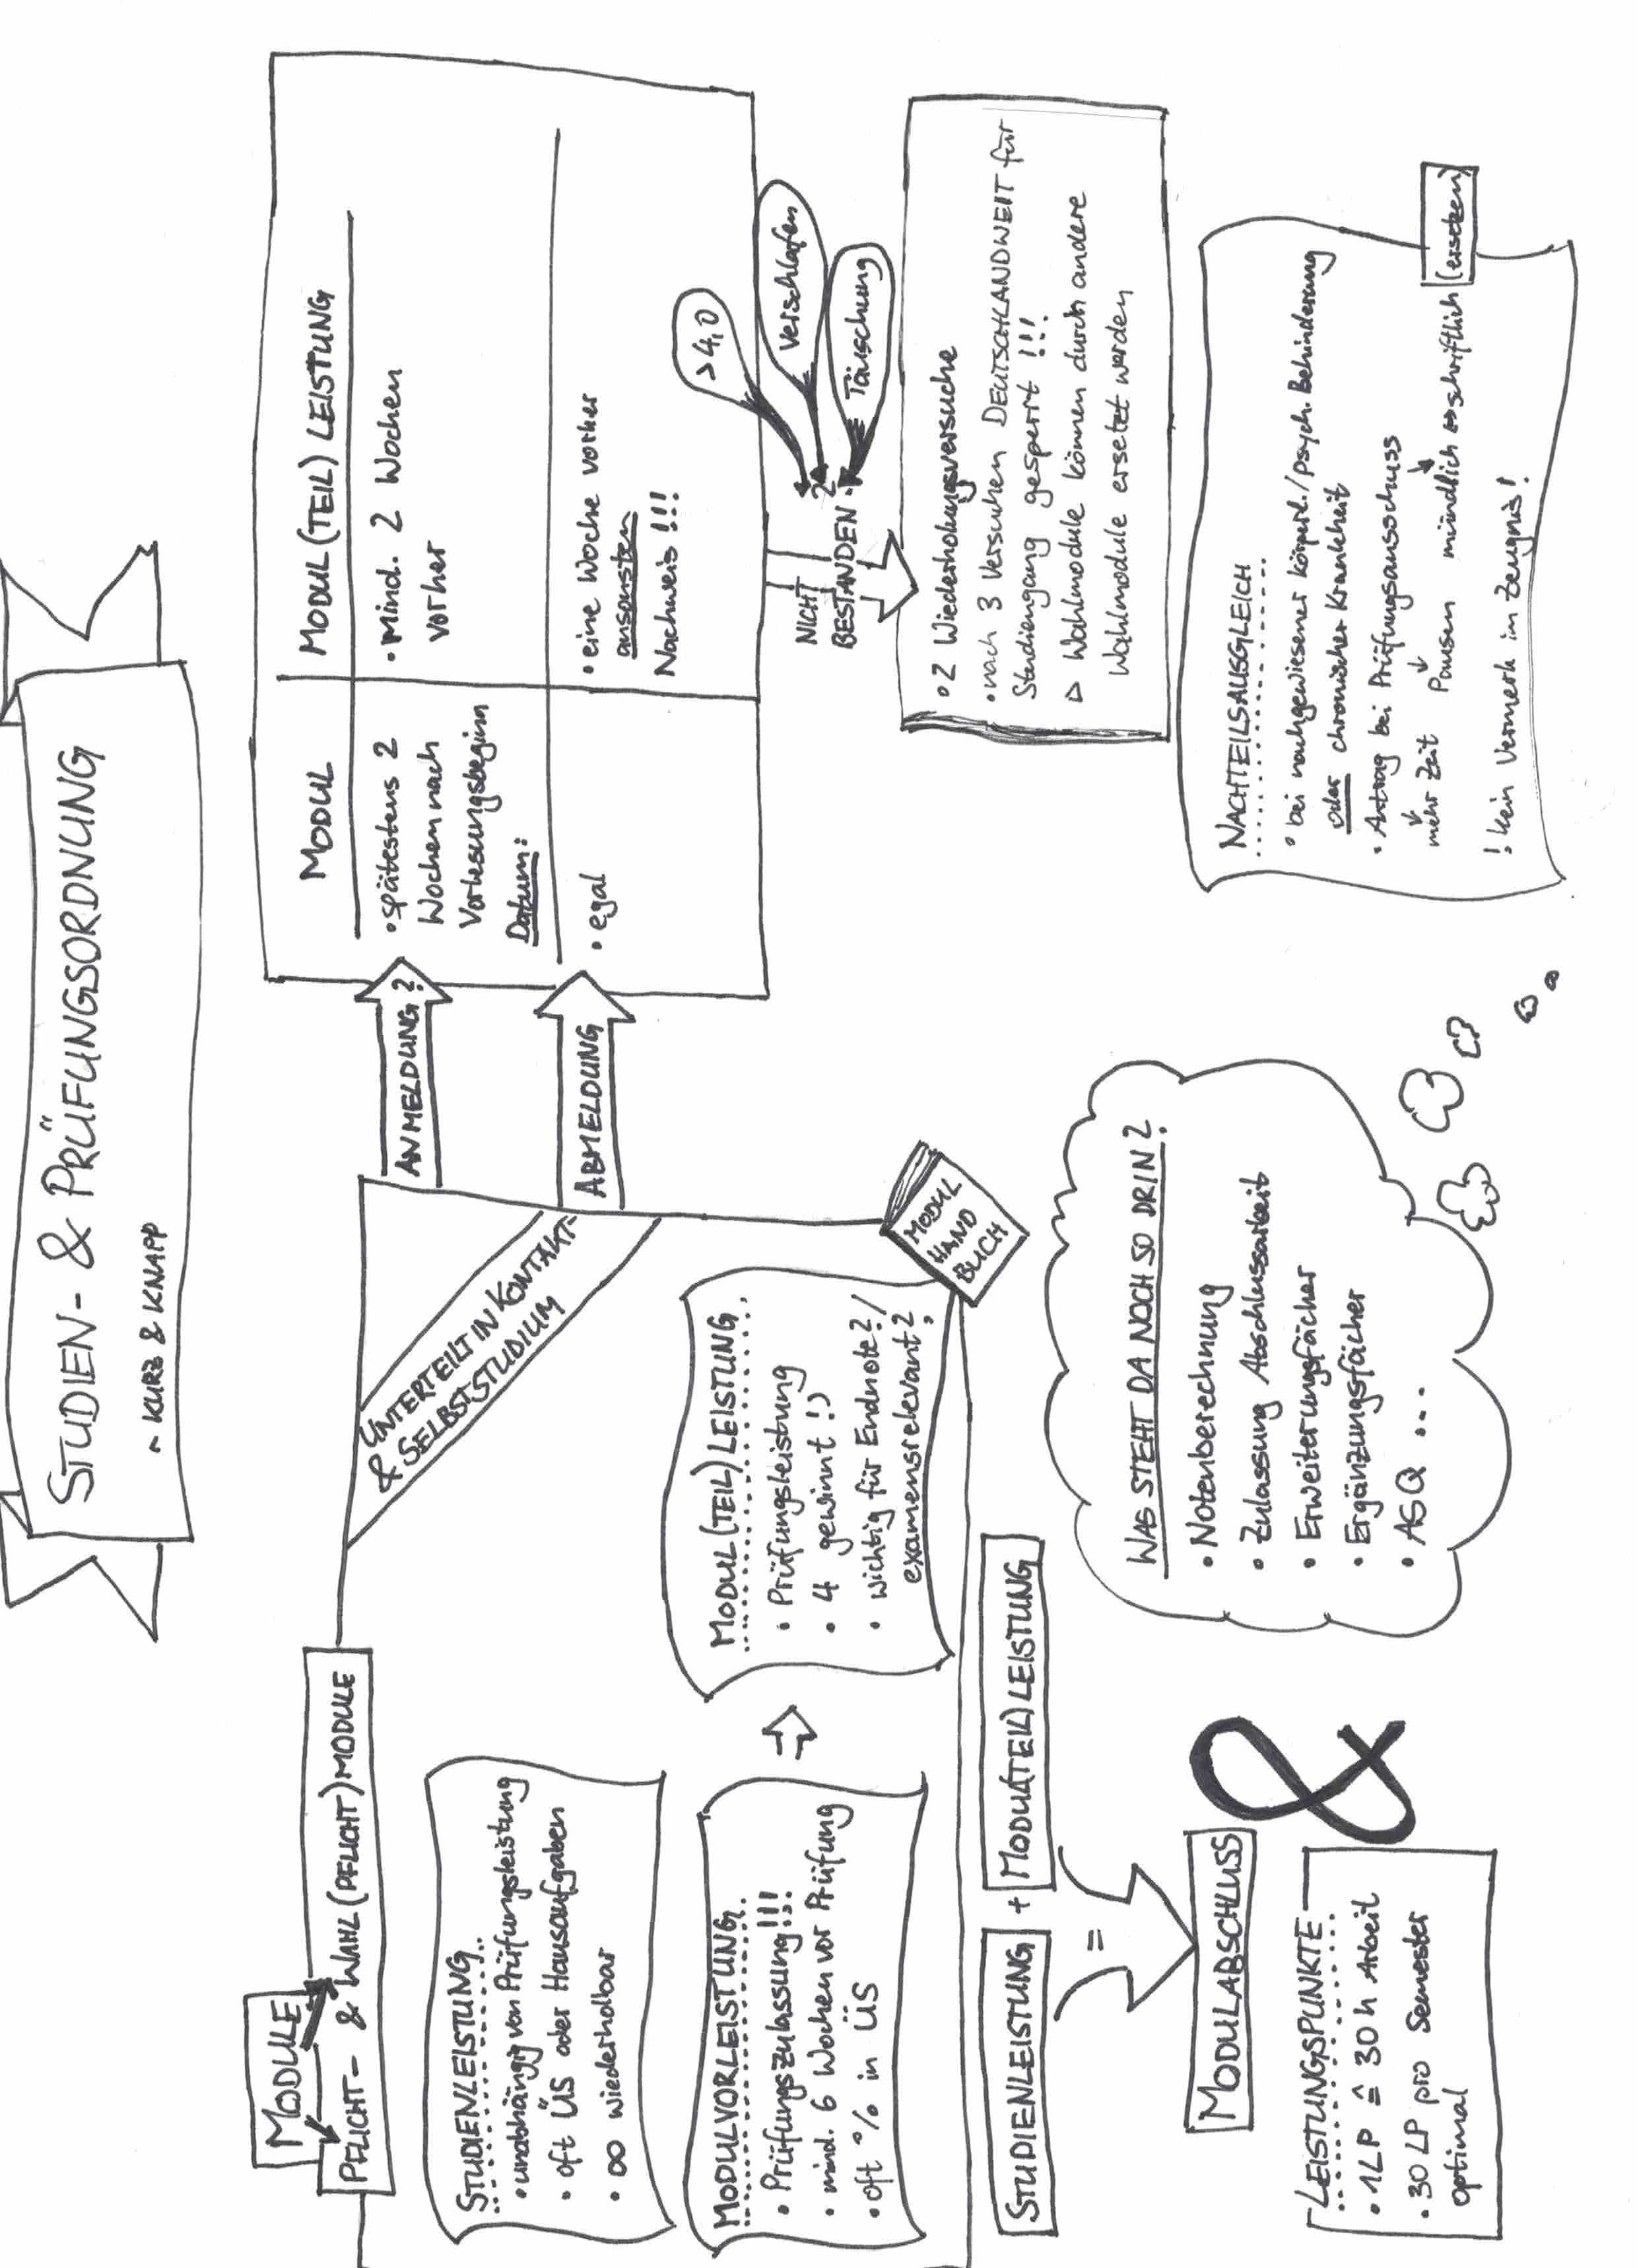
\includegraphics[width=0.90\textwidth]{studiordnung}	
\end{center}

\section{Studiengänge}

Im folgenden Auszüge aus den Modulhandbüchern und Empfehlungen aus den Regelstudienplänen.
Außerdem Ansprechpartner für Fragen und \textquote{Sonderwünsche}.
Fragen können immer auch an den FSR gerichtet werden.

\subsection{Studienberater}
\subsubsection{Mathematik/Wirtschaftsmathematik}
Dr.\ Hans-Georg Rackwitz \\
Theodor-Lieser-Str.~5, Raum~127 \\
Telefon: +49\,345\,55\,24608\\
E-Mail: \email{hans-georg.rackwitz@mathematik.uni-halle.de}\\

\subsubsection{Informatik/Bioinformatik}
Apl.\ Prof.\ Dr.\ Klaus Reinhardt \\
Von-Seckendorff-Platz~1, Raum~2.10 \\
Telefon: +49\,345\,55\,24770 \\
E-Mail: \email{klaus.reinhardt@informatik.uni-halle.de}

\subsubsection{Lehramt}
Zentrum für Lehrerbildung \\
Dr. Marie-Theres Müller \\
Dachritzstraße~12, Raum~205 \\
Telefon: +49\,345\,55\,21717 \\
E-Mail: \email{zlb@uni-halle.de}

\newpage

\section{Studiengangsübersichten}

\subsection{Informatik}
\label{studiengang_informatik}

\subsubsection{Regelstudienplan}
\begin{singlespace}
	\begin{small}
		\begin{longtabu} to \textwidth {X|r@{\hspace{0.75em}}r@{\hspace{0.75em}}r@{\hspace{0.75em}}r@{\hspace{0.75em}}r@{\hspace{0.75em}}r|r}
			\toprule
			\textbf{Modul}&\multicolumn{6}{l|}{\textbf{LP pro Semester}}&\textbf{LP}\\
			& 1. & 2. & 3. & 4. & 5. & 6. &\\
			\midrule
			\endfirsthead
			\midrule
			\textbf{Modul}&\multicolumn{6}{l|}{\textbf{LP pro Semester}}&\textbf{LP}\\
			& 1. & 2. & 3. & 4. & 5. & 6. &\\
			\midrule
			\endhead
			\midrule
			\endfoot
			\bottomrule
			\endlastfoot
			\multicolumn{8}{l}{\textbf{Informatik-Grundlagen}} \\
			Objektorientierte Programmierung & 5 & & & & & & 5 \\ 
			Einführung in die Rechnerarchitektur & 5 & & & & & & 5 \\ 
			Mathematische Grundlagen der Informatik \& Konzepte der Modellierung & 7 & 8 & & & & & 15 \\ 
			Einführung in Betriebssysteme & & 5 & & & & & 5 \\ 
			Einführung in die technische Informatik & & 5 & & & & & 5 \\ 
			Datenstrukturen \& effiziente Algorithmen~I & & 5 & & & & & 5 \\ 
			Konzepte der Programmierung & & & 5 & & & & 5 \\ 
			Automaten \& Berechenbarkeit & & & & 10 & & & 10 \\
			\midrule
			\multicolumn{8}{l}{\textbf{Mathematik}} \\
			Diskrete Strukturen, lineare Algebra \& Analysis (Mathe B) & 8 & 7 & & & & & 15 \\ 
			Einführung in Data Science & & & & 5 & & & 5 \\
			\midrule
			\multicolumn{8}{l}{\textbf{Informatik-Vertiefung}} \\
			Einführung in Datenbanken & & & 5 & & & & 10 \\ 
			Datenstrukturen \& effiziente Algorithmen~II & & & 5 & & & & 5 \\ 
			Einführung in die Rechnernetze \& verteilte Systeme & & & & & 5 & & 5 \\ 
			Softwaretechnik & & & 5 & & & & 5 \\ 
			Einführung in die Bildverarbeitung & & & & 5 & & & 5 \\ 
			Gestaltung \& Durchführung von Fachvorträgen in der Informatik & & & & & 5 & & 5 \\ 
			Projektpraktikum & & & & 5 & 10 & & 15 \\
			\midrule
			\multicolumn{8}{l}{\textbf{Anwendungsfach, ASQ, Wahlpflicht}} \\
			Anwendungsfach & & & 5 & 5 & 5 & & 15 \\ 
			„Spezialisierung“\,/\,Wahlpflicht & & & 5 & & & 10 & 15 \\ 
			Allgemeine Schlüsselqualifikationen (ASQ) & 5 & & & & 5 & 5 & 10 \\
			\midrule
			\textbf{Bachelorarbeit} & & & & & & 15 & 15 \\
		\end{longtabu}
	\end{small}
\end{singlespace}

\subsection{Bioinformatik}
\label{studiengang_bioinformatik}

\subsubsection{Regelstudienplan}
\begin{singlespace}
	\begin{small}
		\begin{longtabu} to \textwidth {X|r@{\hspace{0.75em}}r@{\hspace{0.75em}}r@{\hspace{0.75em}}r@{\hspace{0.75em}}r@{\hspace{0.75em}}r|r}
			\toprule
			\textbf{Modul}&\multicolumn{6}{l|}{\textbf{LP pro Semester}}&\textbf{LP}\\
			& 1. & 2. & 3. & 4. & 5. & 6. &\\
			\midrule
			\endfirsthead
			\midrule
			\textbf{Modul}&\multicolumn{6}{l|}{\textbf{LP pro Semester}}&\textbf{LP}\\
			& 1. & 2. & 3. & 4. & 5. & 6. &\\
			\midrule
			\endhead
			\midrule
			\endfoot
			\bottomrule
			\endlastfoot
			\multicolumn{8}{l}{\textbf{Pflichtbereich Informatik}}\\ 
			Objektorientierte Programmierung & 5 & & & & & & 5 \\
			Grundlagen der Bioinformatik & 8 & 7 & & & & & 15 \\ 
			Datenstrukturen \& effiziente Algorithmen~I & & 5 & & & & & 5 \\ 
			Enführung in Datenbanken & & & 5 & & & & 10 \\ 
			Softwaretechnik & & & 5 & & & & 5 \\ 
			Algorithmen auf Sequenzen~I & & & & 5 & & & 5 \\ 
			Spezielle Probleme der Bioinformatik & & & & 5 & & & 5 \\ 
			Gestaltung \& Durchführung von Fachvorträgen in der Bioinformatik & & & & & 5 & & 5 \\
			Statistische Datenanalyse \& Maschinelles Lernen in der Bioinformatik~I & & & & & 5 & & 5 \\ 
			\midrule
			\multicolumn{8}{l}{\textbf{Pflichtbereich Mathematik}}\\ 
			Diskrete Strukturen, lineare Algebra \& Analysis (Mathe B) & 7 & 8 & & & & & 15 \\ 
			Einführung in Data Science & & & & 5 & & & 5 \\ 
			\midrule
			\multicolumn{8}{l}{\textbf{Pflichtbereich Biologie}}\\ 
			Biologie für Bioinformatiker~I (Zellbiologie, Botanik) & 8 & & & & & & 5 \\ 
			Biologie für Bioinformatiker~II (Mikrobiologie, Ökologie) & & 7 & & & & & 5 \\ 
			Biologie für Bioinformatiker~III (Genetik, Zoologie) & & & 10 & & & & 5 \\ 
			\midrule
			\multicolumn{8}{l}{\textbf{Pflichtbereich Biochemie}}\\
			Allgemeine Biochemie für Bioinformatiker & & & 10 & & & & 10 \\ 
			\midrule
			\multicolumn{8}{l}{\textbf{Pflichtbereich Chemie}}\\ 
			Organische Chemie im Nebenfach (OC-N) & 2 & 3 & & & & & 10 \\ 
			Physikalische Chemie für die Bioinformatik (PC-N~VI) & & & & 5 & & & 5 \\ 
			\midrule
			\multicolumn{8}{l}{\textbf{Pflichtbereich ASQ}}        \\ 
			Allgemeine Schlüsselqualifikationen & & 5 & 5 & & & & 10 \\ 
			\midrule
			\textbf{Bachelorarbeit} & & & & & & 15 & 15 \\
		\end{longtabu}
	\end{small}
\end{singlespace}

\subsubsection{Wahlpflichtmodule}
Hinzu kommen Wahlpflichtmodule aus den Bereichen Informatik und Biowissenschaften mit jeweils 10~LP und 15LP:\\*
\begin{singlespace}
	\begin{small}
		\begin{longtabu} to \textwidth {X|r}
			\toprule
			\textbf{Modul} & \textbf{LP} \\
			\midrule
			\endfirsthead
			\midrule
			\textbf{Modul} & \textbf{LP} \\
			\midrule
			\endhead
			\midrule
			\endfoot
			\bottomrule
			\endlastfoot
			\multicolumn{2}{l}{\textbf{Wahlbereich Informatik}}           \\
			Automaten \& Berechenbarkeit & 10 \\ 
			Big Data Analytics & 5 \\ 
			Bioinformatikpraktikum & 5 \\ 
			Datenbank-Programmierung & 5 \\ 
			Datenstrukturen \& effiziente Algorithmen~II & 5 \\ 
			Einführung in Betriebssysteme & 5 \\ 
			Einführung in die Bildverarbeitung & 5 \\ 
			Einführung in Rechnerarchitektur & 5 \\ 
			Einführung in Rechnernetze \& verteilte Systeme & 5 \\ 
			Formale Sprachen/Petrinetze & 5 \\ 
			Grundlagen benutzerfreundlicher Schnittstellen & 5 \\ 
			Grundlagen des WWW & 5 \\ 
			Introduction to Biodiversity Informatics & 5 \\ 
			Komponenten- \& Servicebasierte Software & 5 \\ 
			Konzepte der Programmierung & 5 \\ 
			Modellierung mit abstrakten Datentypen \& Logik & 5 \\ 
			Projektpraktikum (FSQ-Modul) & 15 \\ 
			Theorie der Datensicherheit & 5 \\ 
			\midrule
			\multicolumn{2}{l}{\textbf{Wahlbereich Biowissenschaften}} \\
			Molekulargenetik der Nutzpflanzen~I & 5 \\
			Einführung in die Toxikologie & 5 \\ 
			Grundlagen Genetik & 5 \\ 
			Molekularbiologie in der Tierzucht & 5 \\ 
			Biochemie \& Biotechnologie für Bioinformatiker (Fortgeschrittene) & 10 \\ 
			Pflanzenphysiologie Bioinformatiker & 5 \\ 
			Ökologiepraktikum & 5 \\ 
			Tierphysiologie für Bioinformatiker & 5 \\ 
			Populationsgenetik für Bioinformatiker & 5 \\ 
			Spezielle Mikrobiologie für Bioinformatiker & 5 \\ 
			Biogeographie & 5 \\ 
			Biophysikalische Chemie im Nebenfach (BioPC-N~I) & 5 \\ 
			Bioorganische Chemie im Nebenfach (BioOC-N) & 5 \\ 
			Angewandte Cheminformatik für die Bioinformatik (BioOC-N) & 5 \\
		\end{longtabu}
	\end{small}
\end{singlespace}

\subsection{Informatik Lehramt}
\label{studiengang_infolehramt}

\subsubsection{Regelstudienplan}

\begin{singlespace}
	\begin{small}
		\begin{longtabu} to \textwidth {X|l|r}
			\toprule
			\textbf{Modul} & \textbf{Semester} & \textbf{LP} \\
			\midrule
			\endfirsthead
			\midrule
			\textbf{Modul} & \textbf{Semester} & \textbf{LP} \\
			\midrule
			\endhead
			\midrule
			\endfoot
			\bottomrule
			\endlastfoot
			\multicolumn{3}{l}{\textbf{Pflichtmodule Informatik}}\\
			Objektorientierte Programmierung & 1. & 5 \\
			Einführung in Rechnerarchitektur & 1. & 5 \\
			Mathematische Grundlagen der Informatik \& Konzepte der Modellierung & 1.\& 2. & 15 \\
			Datenstrukturen \& effiziente Algorithmen I & 2./4 & 5. \\
			Technische Informatik, Betriebssysteme \& Rechnernetze (Lehramt) & 3. & 5 \\
			Konzepte der Programmierung & 3. & 5 \\
			Datenbanken I & 3.\,/\,5.\,/\,7. & 10 \\
			Automaten \& Berechenbarkeit* & 4.\,/\,6. & 10 \\
			Softwaretechnik (Lehramt) & 5. & 5 \\
			Informatik \& Gesellschaft & \(\geq\) 5. & 5 \\
			\midrule
			\multicolumn{3}{l}{\textbf{Wahlmodule Informatik}}\\
			Algorithmen auf Sequenzen I & \(\geq\) 5. & 5 \\
			Datenstrukturen \& effiziente Algorithmen II & \(\geq\) 5. & 5 \\
			Einführung in die Bildverarbeitung & \(\geq\) 5. & 5 \\
			Einführung in die Computergraphik & \(\geq\) 5. & 5 \\
			Einführung in die KI & \(\geq\) 5. & 5 \\
			Einführung in Rechnernetze \& verteilte Systeme & \(\geq\) 5. & 5 \\
			Grundlagen des WWW & \(\geq\) 5. & 5 \\
			Komponenten- \& serviceorientierte Software & \(\geq\) 5. & 5 \\
			Theorie der Datensicherheit & \(\geq\) 5. & 5 \\
			\midrule
			\multicolumn{3}{l}{\textbf{Fachdidaktik Informatik}}\\
			Didaktik der Informatik \(\geq\) & 3.\,/\,4. & 5 \\
			Didaktik der Informatik CDE & \(\geq\) 4. & 5 \\
			Didaktik der Informatik FG & \(\geq\) 5. & 5 \\
		\end{longtabu}
	\end{small}
\end{singlespace}
Das mit * gekennzeichnete Modul sowie die Wahlmodule sind nur für die LAGs zu belegen. Von den Wahlmodulen sind von den LAGs ein bzw. zwei Fächer, falls Informatik das erste Fach ist, zu belegen.

\subsection{Mathematik}
\label{studiengang_mathematik}

\subsubsection{Regelstudienplan}

\begin{singlespace}
	\begin{small}
		\begin{longtabu} to \textwidth {X|r@{\hspace{0.75em}}r@{\hspace{0.75em}}r@{\hspace{0.75em}}r@{\hspace{0.75em}}r@{\hspace{0.75em}}r|r}
			\toprule
			\textbf{Modul}&\multicolumn{6}{l|}{\textbf{LP pro Semester}}&\textbf{LP}\\
			& 1. & 2. & 3. & 4. & 5. & 6. &\\
			\midrule
			\endfirsthead
			\midrule
			\textbf{Modul}&\multicolumn{6}{l|}{\textbf{LP pro Semester}}&\textbf{LP}\\
			& 1. & 2. & 3. & 4. & 5. & 6. &\\
			\midrule
			\endhead
			\midrule
			\endfoot
			\bottomrule
			\endlastfoot
			Analysis~I+II & 9 & 9 & & & & & 18\\
			Lineare Algebra~I+II & 9 & 9 & & & & & 18\\
			Informatik & 5 & 5 & & & & & 10\\
			Numerik~I+II & & 9 & 9 & & & & 18\\
			Analysis~III & & & 9 & & & & 9\\
			Algebra & & & 9 & & & & 9\\
			Maßtheorie & & & & 8 & & & 8\\
			Wahrscheinlichkeitstheorie \& Statistik & & & & 8 & & & 8\\
			Funktionalanalysis & & & & & 8 & & 8\\
			Wahlpflichtmodul I & & & & 8 & & & 8\\
			Proseminarund Seminar & & & & 5 & 5 & & 10\\
			Praktikum & & & & 6 & & & 6\\
			Wahlpflichtmodul II & & & & & 15 & & 15\\
			Anwendungsfach & & & 5 & 5 & 5 & 5 & 20\\
			ASQ & 5 & & & & 5 & & 10\\
			\midrule
			\textbf{Bachelorarbeit}& & & & & & 15 & 15\\
		\end{longtabu}
	\end{small}
\end{singlespace}

\subsection{Wirtschaftsmathematik}
\label{studiengang_wima}

\subsubsection{Regelstudienplan}

Die Wirtschaftswissenschaftsmodule sind Platzhalter für die unter der Tabelle aufgeführten Wahlpflichtmodule.

\begin{singlespace}
	\begin{small}
		\begin{longtabu} to \textwidth {X|r@{\hspace{0.75em}}r@{\hspace{0.75em}}r@{\hspace{0.75em}}r@{\hspace{0.75em}}r@{\hspace{0.75em}}r|r}
			\toprule
			\textbf{Modul}&\multicolumn{6}{l|}{\textbf{LP pro Semester}}&\textbf{LP}\\
			& 1. & 2. & 3. & 4. & 5. & 6. &\\
			\midrule
			\endfirsthead
			\midrule
			\textbf{Modul}&\multicolumn{6}{l|}{\textbf{LP pro Semester}}&\textbf{LP}\\
			& 1. & 2. & 3. & 4. & 5. & 6. &\\
			\midrule
			\endhead
			\midrule
			\endfoot
			\bottomrule
			\endlastfoot
			\multicolumn{8}{l}{\textbf{Pflichtmodule}}\\
			Analysis~I+II & 9 & 9 & & & & & 18\\
			Lineare Algebra~I+II & 9 & 9 & & & & & 18\\
			Informatik & 10 & 5 & & & & & 15\\
			ASQ & & & & & 5 & 5 & 10\\
			Optimierung (2-semestrig)& & 20 & & & & & 20\\
			Analysis III & & & 9 & & & & 9\\
			Maßtheorie & & & & 8 & & & 8\\
			Numerik für Wirtschaftsmathematiker & & & & 8 & & & 8\\
			Wahrscheinlichkeitstheorie \& Statistik & & & & 8 & & & 8\\
			Proseminar \& Seminar & & & & 5 & 5 & & 10\\
			Versicherungsmathematik \& Risikotheorie & & & & & 8 & & 8\\
			Vertiefungsmodul Mathematik & & & & & 5 & & 5\\
			Wirtschaftswissenschaftsmodule & & & 10 & 5 & 5 & 5 & 25\\
			Praktikum & & & & 8 & & & 8\\
			\midrule
			\textbf{Bachelorarbeit}& & & & & & 15 & 15\\
		\end{longtabu}
	\end{small}
\end{singlespace}

\subsubsection{Wirtschaftswissenschaftsmodule}

\begin{singlespace}
	\begin{small}
		\begin{longtabu} to \textwidth {X|r}
			\toprule
			\textbf{Modul} & \textbf{LP} \\
			\midrule
			\endfirsthead
			\midrule
			\textbf{Modul} & \textbf{LP} \\
			\midrule
			\endhead
			\midrule
			\endfoot
			\bottomrule
			\endlastfoot
			Grundlagen der BWL & 5\\
			Grundlagen der VWL & 5\\
			Mikroökonomik I & 5\\
			Mikroökonomik II & 5\\
			Makroökonomik I & 5\\
			Makroökonomik II & 5\\
			Wertschöpfungsmanagement & 5\\
			Internes Rechnungswesen & 5\\
			Produktion \& Logistik & 5\\
			Investition \& Finanzierung & 5\\
			Entscheidungs- \& Spieltheorie & 5\\
		\end{longtabu}
	\end{small}
\end{singlespace}

\subsection{Mathematik Lehramt}
\label{studiengang_lehramt}

\subsubsection{Regelstudienplan Gymnasium}
\label{studiengang_lag}

Bei den mit * gekennzeichneten Teilgebieten muss jeweils nur ein Modul besucht werden.

\begin{singlespace}
	\begin{small}
		\begin{longtabu} to \textwidth {X|l|r}
			\toprule
			\textbf{Modul} & \textbf{Semester} & \textbf{LP} \\
			\midrule
			\endfirsthead
			\midrule
			\textbf{Modul} & \textbf{Semester} & \textbf{LP} \\
			\midrule
			\endhead
			\midrule
			\endfoot
			\bottomrule
			\endlastfoot
			Analysis~I \& II & 1.\,--\,2. & 15\\
			Lineare Algebra & 1.\,--\,2. & 15\\
			Wahrscheinlichkeitstheorie \& Statistik & 4.& 6\\
			Proseminar & 4.& 5\\
			Grundl. der numerischen Mathematik & \(\geq\) 3.& 5\\
			Algebra & \(\geq\) 3.& 7\\
			Fachseminar & 5.& 5\\
			Vertiefungsmodul (nur wenn Erstfach)& \(\geq\) 3.& 5\\
			Mathematikdidaktik AB & 3.\,--\,4. & 5\\
			Mathematikdidaktik CDE & 4.\,--\,5. & 5\\
			Mathematikdidaktik FG & 6.\,--\,8. & 5\\
			\midrule
			\multicolumn{3}{l}{\textbf{Geometrie*}}\\
			Geometrie & 5.\,/\,7. & 7\\
			Differentialgeometrie & 5.\,/\,7. & 7\\
			\midrule
			\multicolumn{3}{l}{\textbf{Grundlagen*}}\\
			Geschichte der Mathematik & \(\geq\) 4.& 5\\
			Grundlagen der Mathematik & \(\geq\) 4.& 5\\
			\midrule
			\multicolumn{3}{l}{\textbf{Analysis/Numerik*}}\\
			Funktionentheorie & \(\geq\) 5.& 5\\
			Gewöhnl. Differentialgl.& \(\geq\) 5.& 5\\
			Theorie u. Num. gewöhnl. Dgl.& \(\geq\) 5.& 5\\
		\end{longtabu}
	\end{small}
\end{singlespace}

\subsubsection{Regelstudienplan Sekundarschule}
\label{studiengang_las}

Bei dem mit * gekennzeichneten Teilgebiet müssen zwei Module besucht werden.

\begin{singlespace}
	\begin{small}
		\begin{longtabu} to \textwidth {X|l|r}
			\toprule
			\textbf{Modul} & \textbf{Semester} & \textbf{LP} \\
			\midrule
			\endfirsthead
			\midrule
			\textbf{Modul} & \textbf{Semester} & \textbf{LP} \\
			\midrule
			\endhead
			\midrule
			\endfoot
			\bottomrule
			\endlastfoot
			Lineare Algebra & 1.\,--\,2. & 15\\
			Elemente der Mathematik & 1.\,--\,2. & 5\\
			Analysis~I & 3.& 10\\
			Elemente der Kombinatorik \& Stochastik & 5.& 5\\
			Elemente der Geometrie & 3.\,/\,5. & 5\\
			Proseminar & \(\geq\) 4. & 5 \\
			Algebra & 5. & 5\\
			Vertiefungsmodul (nur wenn Erstfach)& \(\geq\) 4.& 5\\
			Mathematikdidaktik AB & 3.\,--\,4. & 5\\
			Mathematikdidaktik CDE & 4.\,--\,5. & 5\\
			Mathematikdidaktik FG & 6.\,--\,8. & 5\\
			\midrule
			\multicolumn{3}{l}{\textbf{Mathematik*}}\\
			Analysis~II & \(\geq\) 4.  & 5\\
			Geschichte der Mathematik & \(\geq\) 4.  & 5\\
			Grundlagen der numerischen Mathematik & \(\geq\) 5.  & 5\\
			Mathematische Biologie & \(\geq\) 4.  & 5\\
			Funktionentheorie & \(\geq\) 5.  & 5\\
			Geometrie & \(\geq\) 5.  & 5\\
			Diskrete Mathematik & \(\geq\) 5. & 5\\
		\end{longtabu}
	\end{small}
\end{singlespace}
